\documentclass{article}
\usepackage[utf8]{inputenc}

\title{CS246 Homework 3 Answers}
\author{Charlie Zhang}
\date{Feb 2013}

\usepackage{natbib}
\usepackage{float}
\usepackage{graphicx}
 \usepackage{indentfirst}
\usepackage{mathtools}
\linespread{1.3}

\begin{document}

\maketitle
\section{Question 1 -- Latent Features for Recommendations}


\subsection{(a)}
$\epsilon_{iu} = r_{iu} - q_i * p_u^T$

$q_i \leftarrow q_i + \eta(\epsilon_{iu}p_u - \lambda q_i)$

$p_u \leftarrow p_u + \eta(\epsilon_{iu}q_i - \lambda p_u)$

Where $\eta$ is the learning rate.

\subsection{(b)}
\begin{figure}[H]
\centering
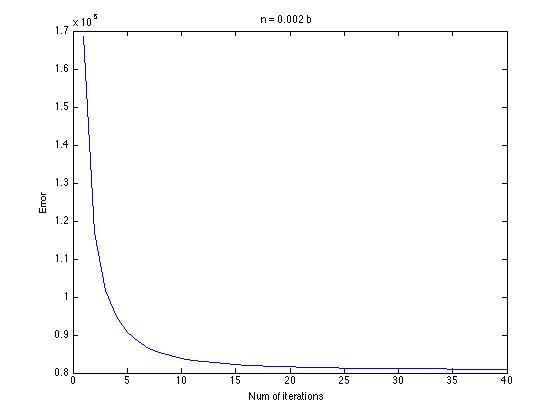
\includegraphics[scale=0.5]{EAsOfIterationEta0002.jpg}
\caption{ Error in first 40 iterations with $\eta=0.002$: }
\label{}
\end{figure}


\subsection{(c)}
True statements are: \\
B, D, H


\subsection{(d)}
TODO

\section{Question 2 -- PageRank Computation}
\subsection{(a)}
$r - r^{(k)} = \beta Mr - \beta Mr^{(k-1)} \\
=\beta M(r - r^{(k-1)}) \\
=\beta^2M^2(r - r^{(k-2)}) \\
=... \\
=\beta^kM^k(r - r^{(0)})$ \\
$M$ is stochastic, $\|M^kr\|_1 <= 1, \|M^kr^{(0)}\|_1 <= 1$ \\
So $\|r - r^{(k)}\|_1 <= \|\beta^k M^kr\|_1 + \|\beta^k M^kr^{(0)}\|_1 <= 2\beta^k$

\subsection{(b)}
Let $I$ be the number of iterations. \\
$\|r - r^{(I)}\|_1<= 2\beta^I <= \delta$\\
$I >= \log_\beta (\delta/2) = \frac{\log (2/\delta)}{\log (1/\beta)}$
We need iterate through every edge one time for each iteration. So total running time is: \\
$Im = m \frac{\log (2/\delta)}{\log (1/\beta)} = O({\frac{m}{\log (1/\beta)}})$



\subsection{(c)}
TODO

\subsection{(d)}
TODO
\end{document}